
\documentclass[10pt]{article}
\usepackage[top=20mm, bottom=20mm, left=20mm, right=20mm]{geometry}
\geometry{a4paper}
\geometry{portrait}
\usepackage[utf8]{inputenc}	% Comment out for xelatex; must use with pdflatex
\usepackage[T1]{fontenc}
\usepackage[parfill]{parskip} % Activate to begin paragraphs with an empty line rather than an indent
\usepackage{graphicx}
\usepackage{amsmath}
\usepackage{amssymb}
%\usepackage{fontspec}
\usepackage{epstopdf}
\usepackage{float}
\usepackage[hang]{footmisc}
\usepackage{endnotes}
\usepackage{listingsutf8}
%\restylefloat{table}
\usepackage{xcolor}
\usepackage{colortbl}
%\usepackage{booktabs}
\usepackage{tabu}
\usepackage{caption}
\usepackage{textcomp}
\usepackage{textgreek}
\usepackage{subcaption}
\usepackage{hyperref}
\usepackage[normalem]{ulem}
\usepackage{authblk}
\usepackage[numbers]{natbib}
\usepackage{xr}
\externaldocument{supplementary}

\bibliographystyle{plos2015}


\makeatletter
\def\blx@maxline{77}
\makeatother

\captionsetup[figure]{labelfont=sc}
\captionsetup[table]{labelfont=sc}
\captionsetup[tabu]{labelfont=sc}

\DeclareCaptionType{MPEquation}[][List of equations]
\captionsetup[MPEquation]{labelformat=empty}

\DeclareCaptionType{MPListing}[][List of listings]
\captionsetup[MPListing]{labelformat=empty}

\usepackage{fancyhdr}
\setlength{\headheight}{16pt}
\pagestyle{fancyplain}
\fancyhf{}
%\fancypagestyle{plain}{}
\cfoot[\thepage]{\thepage}

\usepackage{stringenc}
\usepackage{pdfescape}


% Helper for debugging pdflatex errors induced by invalid UTF8 characters:
% output the actual character code causing the issue.

\makeatletter
\renewcommand*{\UTFviii@defined}[1]{%
\ifx#1\relax
\begingroup
% Remove prefix "\u8:"
\def\x##1:{}%
% Extract Unicode char from command name
% (utf8.def does not support surrogates)
\edef\x{\expandafter\x\string#1}%
\StringEncodingConvert\x\x{utf8}{utf16be}% convert to UTF-16BE
% Hexadecimal representation
\EdefEscapeHex\x\x
% Enhanced error message
\PackageError{inputenc}{Unicode\space char\space \string#1\space
(U+\x)\MessageBreak
not\space set\space up\space
for\space use\space with\space LaTeX}\@eha
\endgroup
\else\expandafter
#1%
\fi
}
\makeatother

% Make multi-paragraph footnotes align nicely on the left
\setlength\footnotemargin{10pt}

% Do not display an automatic Notes heading for endnotes, as they are contained
% by a Manuscripts section with a heading that has possibly been edited by the user
\def\enoteheading{}

% Apply footnote and endnote numbering schemes (decimal, lowercase roman etc.)
\renewcommand{\thefootnote}{\arabic{footnote}}
\renewcommand{\theendnote}{\arabic{endnote}}
% Adjust endnotes to use normal-sized numbering and text
\renewcommand{\enotesize}{\normalsize}
\renewcommand\enoteformat{%
  \raggedright
  \leftskip=1.8em
  \makebox[0pt][r]{\theenmark. \rule{0pt}{\dimexpr\ht\strutbox+\baselineskip}}%
}

\begin{document}
\title{Nested Stochastic Block Models Applied to the Analysis of Single Cell Data}
\author[1,2]{Leonardo Morelli}
\author[1,3]{Valentina Giansanti}
\author[1]{Davide Cittaro}
\affil[1]{Center for Omics Sciences, IRCCS San Raffaele Institute, Milan, Italy}
\affil[2]{Universit\`{a} Vita-Salute San Raffaele, Milan, Italy} 
\affil[3]{Department of Informatics, Systems and Communication, University of Milano-Bicocca, Milan, Italy}
\maketitle

\section*{Abstract}

Single cell profiling has been proven to be a powerful tool in molecular biology to understand the complex behaviours of heterogeneous system. While properties of single cells is the primary endpoint of such analysis, these are typically clustered to underpin the common determinants that can be used to describe functional properties of the cell mixture under investigation. Several approaches have been proposed to identify cell clusters; while this is matter of active research, one popular approach is based on community detection in neighbourhood graphs by optimisation of modularity. In this paper we propose an alternative solution to this problem, based on Stochastic Block Models; we show a threefold advantage of our approach as it is able to correctly identify cell groups, it returns a meaningful hierarchical structure and, lastly, it provides a statistical measure of association between cells and the assigned clusters.


\section*{Background}

Transcriptome analysis at single cell level by RNA sequencing (scRNA-seq) is a technology growing in popularity and applications \cite{svensson_2018}. It has been applied to study the biology of complex tissues \cite{guo_2018, ventotormo_2018}, tumor dynamics \cite{rozenblattrosen_2020, tirosh_2016, patel_2014, neftel_2019}, development \cite{rosenberg_2018, wagner_2018} and to describe whole organisms \cite{plass_2018, regev_2017}.

A key step in the analysis of scRNA-seq data and, more in general, of single cell data, is the identification of cell populations, that is groups of cells sharing similar properties. Several approaches have been proposed to achieve this task, based on well established clustering techniques \cite{wang_2017, lin_2017}, consensus clustering \cite{huh_2020, kiselev_2017, Ranjan_2021} and deep learning \cite{li_2020}; many more have been recently reviewed \cite{krzak_2019, kiselev_2019} and benchmarked \cite{du_2018}. As the popularity of single cell analysis frameworks Seurat \cite{butler_2018} and Scanpy \cite{wolf_2018} raised, methods based instead on graph partitioning became the \emph{de facto} standards. Such methods require the construction of a cell neighbourhood graph (\emph{e.g.} by \emph{k }Nearest Neighbours, \emph{k}NN or shared Nearest Neighbors, \emph{s}NN). Encoding cell-to-cell similarities into graphs has practical advantages, as many algorithms for graph analysis can be applied and interpreted in a biological way. A notable example is the analysis of cell trajectories which can be derived from the analysis of random walks on the NN graph (\textcolor{red}{CHECK THIS: it's actually from diffusion maps}; computation of RNA moments in scRNA velocity is also based on the NN graph structure \cite{Bergen_2020}. Arguably, the biggest utility of NN structure is the possibility to identify cell groups by partitioning the graph into communities; the latter step is typically performed using the Louvain method \cite{blondel_2008}, a fast algorithm for optimisation of graph modularity. While fast, this method does not guarantee that small communities in large networks are well defined. To overcome its limits, a more recent approach, the Leiden algorithm \cite{traag_2019}, has been implemented and it has been quickly adopted in the analysis of single cell data, for example by Scanpy \cite{wolf_2018} and PhenoGraph \cite{levine_2015}. In addition to Newman's modularity \cite{newman_2004}, other definitions currently used in single cell analysis make use of a resolution parameter \cite{traag_2011, reichardt_2006}. In lay terms, resolution works as a threshold on the density within communities: lowering the resolution results in less and sparser communities and \emph{viceversa}. Identification of an appropriate resolution has been recognised as a major issue \cite{lhnemann_2020}, also because it requires the definition of a mathematical property (clusters) over biological entities (the cell groups), with little formal description of the latter. In addition, the larger the dataset, the harder is to identify small cell groups, as a consequence of the well-known resolution limit \cite{fortunato_2007}. Moreover, it has been demonstrated that random networks can have modularity \cite{guimer_2004} and its optimisation is incapable of separating actual structure from those arising simply of statistical fluctuations of the null model. Additional solutions to cell group identification from neighbourhood graphs have been proposed, introducing resampling techniques \cite{baran_2019, Tang_Sackton_2020} or clique analysis \cite{xu_2015}. Lastly, it has been proposed that high resolution clustering, \emph{e.g.} obtained with Leiden or Louvain methods, can be refined in agglomerative way using machine learning techniques \cite{miao_2020}.

An alternative solution to community detection is the Stochastic Block Model, a generative model for graphs organized into communities \cite{holland_1983}. In this scenario, identification of cell groups requires the estimation of the proper parameters underlying the observed neighbourhood graph. According to the microcanonical formulation \cite{peixoto_2017}, the parameters are node partitions into groups and the matrix of edge counts between groups themselves. Under this model, nodes belonging to the same group have the same probability to be connected with other nodes. It is possible to include node degree among the model parameters \cite{karrer_2011}, to account for heterogeneity of degree distribution of real-world graphs. A Bayesian approach to infer parameters has been developed \cite{peixoto_2013} and implemented in the \emph{graph-tool} python library (\href{https://graph-tool.skewed.de}{https:/\slash graph-tool.skewed.de}). There, a generative model of network $\boldsymbol A$ has a probability $P(\boldsymbol A|\boldsymbol\theta, \boldsymbol b)$ where \textbf{$\boldsymbol\theta$} is the set of parameters and \textbf{\emph{$\boldsymbol b$}} is the set of partitions. The likelihood of the network being generated by a given partition can be measured by the posterior probability


\begin{MPEquation}[!ht]
\begin{equation}
P(\boldsymbol b | \boldsymbol A) = \frac{P(\boldsymbol A|\boldsymbol\theta, \boldsymbol b)P(\boldsymbol\theta, \boldsymbol b)}{P(\boldsymbol A)}
\end{equation}
\label{MPEquationElement:820CB015-E51E-4C5A-BD9C-70E667B8F73B}
\end{MPEquation}
and inference is performed by maximising the posterior probability. The numerator in this equation can be rewritten exponentiating the description length


\begin{MPEquation}[!ht]
\begin{equation}
\Sigma = -\ln P(\boldsymbol A|\boldsymbol\theta, \boldsymbol b) - \ln P(\boldsymbol\theta, \boldsymbol b)
\end{equation}
\label{MPEquationElement:676396C0-2D6F-4084-89B1-951DE3032087}
\end{MPEquation}

so that inference is performed by minimizing the information required to describe the data (Occam's razor); \emph{graph-tool} is able to efficiently do this by a Markov Chain Monte Carlo approach \cite{peixoto_2014}. SBM itself may fail to identify small groups in large graphs, hence hierarchical formulation has been proposed \cite{peixoto_2014_h}. Under this model, communities are agglomerated at a higher level in a block multigraph, also modelled using SBM. This process is repeated recursively until a graph with a single block is reached, creating a Nested Stochastic Block Model (nSBM).

In this work we propose nSBM for the analysis of single cell data, in particular scRNA-seq data. This approach identifies cell groups in a statistical robust way and, moreover, it is able to determine the likelihood of the grouping, thus allowing model selection. In addition, it is possible to measure the confidence of assignment to groups. \textcolor{red}{We show that such information may be exploited to perfect the notion of cell groups and the identification of markers.}

We developed \emph{schist} (\href{https://github.com/dawe/schist}{https:/\slash github.com\slash dawe\slash schist}), a python library compatible with \emph{scanpy}, to facilitate the adoption of stochastic block models in single-cell analysis.

\section*{Results}

\subsection*{Overview of \emph{schist}}

\emph{schist} is a convenient wrapper to the \emph{graph-tool} python library, written in python and designed to be used with \emph{scanpy}. The most prominent function is \emph{schist.inference.nested\_model()} which takes a \emph{AnnData} object as input and fits a nested stochastic block model on the \emph{k}NN graph built with \emph{scanpy} functions (\emph{e.g.\ scanpy.tools.neighbors()}). When launched with default parameters, \emph{schist} fits a model which maximises the posterior probability of having a set of cell groups (or blocks) given a graph. \emph{schist} then annotates cells in the data object with all the groups found at each level of a hierarchy. Given the large size of the NN graph, it is possible that a single solution represents local minima of the fitting process. In addition, it is possible that multiple solutions are equally acceptable to represent the graph partitioning and a better description is given by the consensus over such solutions \cite{Peixoto_2021_consensus}. To overcome these issues, \emph{schist} fits multiple instances in parallel and returns the inferred consensus model, alongside the marginal probabilities for each cell to belong to a specific group (\emph{cell marginals}). 
In addition to the default Nested Stochastic Block Model, \emph{schist} implements the possibility to fit a Bayesian model able to find statistically significant assortative modules \cite{Zhang_Peixoto_2020}, eliminating the need to set a resolution parameter as required in standard community detection by maximization of modularity.
Once a model has been fitted, \emph{schist} allows to evaluate the difference in entropy given by assigning every cell to every possible group. This step allows to estimate the probability for a cell to belong to a specific group (\emph{cell affinity}). We show that cell affinity may have practical application in common tasks in single cell analysis, such as label transfer.

\subsection*{nSBM does not return artificial cell groupings}

One of the most relevant difference between nSBM and other methods to cluster single cells is that it relies on robust statistical modelling. In this sense, the number of groups identified strictly mirrors the amount of information contained in the data. An important consequence is that absence of information can be properly handled. To show this property we performed a simple experiment on a randomised \emph{k}NN graph. To this end we collected data for 3k PBMC (available as preprocessed data in \emph{scanpy}) and shuffled the edges of the prebuilt \emph{k}NN graph, this to keep the general graph properties unchanged. We tested that the degree distribution does not change after randomisation (Kolmogorov-Smirnov $D=0.0733$, $p=0.703$). We found that the default strategy, based on maximisation of modularity, identifies 24 cell groups, whereas nSBM does not identify any cell group. 

\begin{figure}[H]
\centering
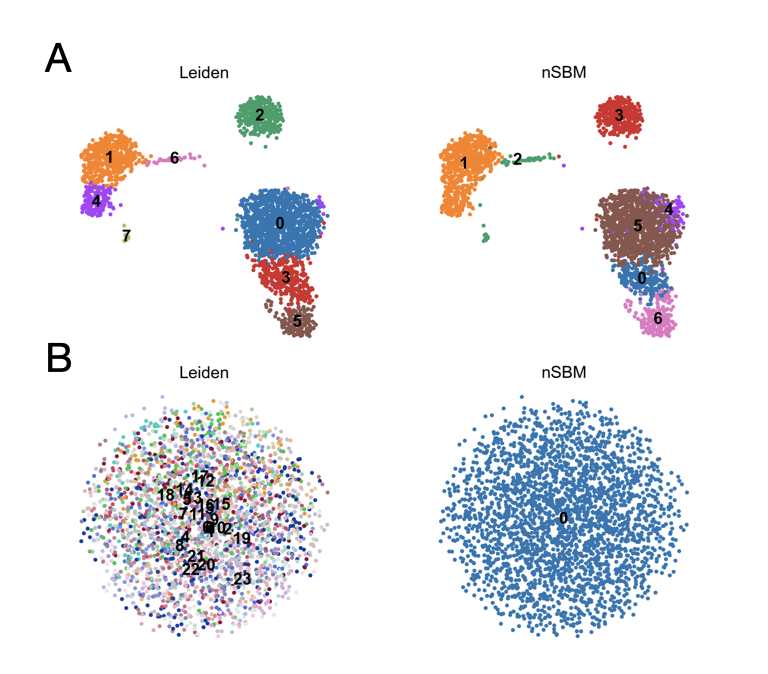
\includegraphics[keepaspectratio,width=\textwidth,height=0.4\textheight]{FIgure_Random.png}
\caption[]{nSBM results for randomised data. (A) UMAP embedding of ~3k PBMC after standard processing with Leiden approach (left) or nSBM (right). Cell grouping is consistent for both the approaches (Adjusted Rand Index $ARI=0.869$). (B) UMAP embedding of the same data after randomisation of \emph{k}NN graph edges. In this case nSBM does not return any cell grouping, while optimisation of modularity finds up to 24 different cell groups}\label{FigureRandom}
\end{figure}

This experiment is a deliberate extreme case. The quality of grouping proposed by a standard approach can be disputed in many ways, and the UMAP embedding indeed reflects the absence of any information. Nevertheless, real-world data may include an unknown amount of random noise. Hence, It is important to identify cell groups that are not artefacts arising from processing and that do not reflect the information contained in the dataset. 

\subsection*{nSBM correctly identifies cell populations}

\textcolor{red}{TO BE UPDATED, possibly with some simulation study}


%To benchmark \emph{schist}, we tested our approach on scRNA-seq mixology data \cite{tian_2019}, in particular on a mixture of 5 cell lines profiled with Chromium 10x platform. At a first evaluation of the UMAP embedding, all lines appear well separated. Only the lung cancer line H1975 shows a certain degree of heterogeneity with some cells being embedded in other cell groups (Fig. \ref{Figure1}A). Inference on the neighbourhood graph is influenced by the graph structure itself, therefore we built multiple graphs changing the number of principal components used in PCA reduction and the number of neighbours in the \emph{k}NN graph. We then calculated the Adjusted Rand Index (\emph{ARI}) between the cell line assignments (ground truth) and the cell groups identified by nSBM at each level. We found a peak of $ARI=0.977$ with 30 principal components (PC) and 30 neighbours. In general, higher number of components and neighbours has a positive impact on the performance (Fig. \ref{Figure1}B). Conversely, if few PCs (10) or neighbors (5) are used, performances degrade, with a minimum $ARI=0.669$ at 20 PCs and 5 neighbours. If fewer PCs are used, a smaller fraction of the total variance, hence less information, is used to build the \emph{k}NN graph; if fewer neighbours are chosen, the graph is sparser and the model is fit from less edges (Fig. S1). Running MCMC algorithm recovers the performances of the majority of the configurations (Fig. S2).

%\begin{figure}[H]
%\centering
%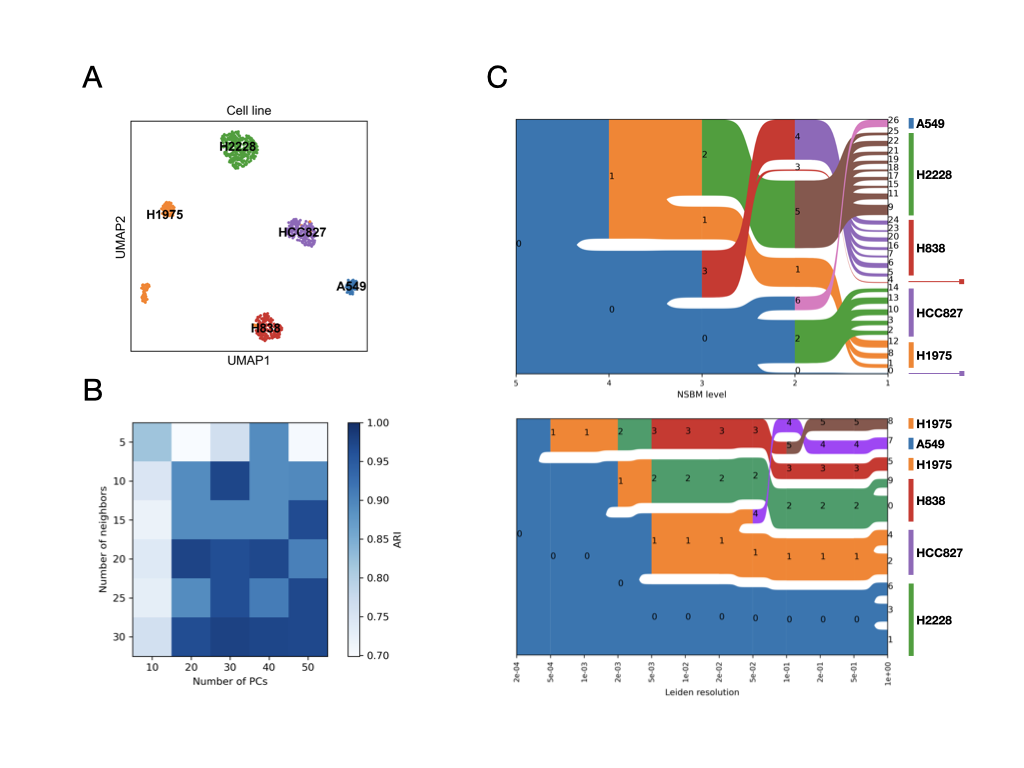
\includegraphics[keepaspectratio,width=\textwidth,height=0.6\textheight]{Figure_1.png}
%\caption[]{\emph{schist} applied to scRNA-seq mixology data. (A) UMAP embedding of 10x Chromium data, cells are colored according to the given cell line in the original paper. A small number of H1975 cells are found in HCC827 and H838 clusters. (B) Heatmap showing the maximal Adjusted Rand Index for different \emph{k}NN graphs. We tested the impact of varying the number of Principal Components and the number of neighbors used in \emph{sc.pp.neighbors()} function in \emph{scanpy}. Adjusted Rand Index between the actual cell lines and the identified groups is shown. Darker blue indicates higher concordance between the model and the ground truth. (C) Alluvial plots showing the hierarchy of cell groups as identified by \emph{schist} (above) or by Leiden method at different resolution thresholds (below). The bars on the right indicate the cell identity; two marks in the \emph{schist} plot indicate two groups of cells discussed in the main text}\label{Figure1}
%\end{figure}

%Analysis of the nSBM hierarchy reveals that five levels are needed to describe the experiment (Fig. \ref{Figure1}C, upper panel), with level 2 properly catching the cell identity ($ARI = 0.977$). In addition to the five major groups, observe two small groups, summing to 11 cells, that were merged to HCC827 and H838 at hierarchy level 3. Interestingly, these groups are enriched in cells whose identity was reassigned from H1975 to H838 or HCC827 in the original paper using Demuxlet \cite{kang_2018}, indicating that nSBM was able to recognise peculiar properties and isolate them. It may be worth mention that the second best ranked group by cell affinity for these 11 cells is the correct group assigned in the original paper, except for a single cell assigned to H2228.
%As a high separation between cell lines is observable, optimisation of modularity by Leiden algorithm is also able to identify cell identities with high precision, given that a proper resolution threshold is set (Fig. \ref{Figure1}C, lower panel); we found that when resolution is set to 0.05 the cell lines are properly separated ($ARI = 0.975$), with the exception of the above mentioned cells.

%These observations show that nSBM is able to perform accurate identification of cell groups, without the need of an arbitrary threshold on the resolution parameter. These data also hint at the possibility to identify rare cell types in larger populations.

\subsection*{Comparison with other methods}

\textcolor{red}{TO BE FILLED with SSCAF?}


\subsection*{Hierarchy modelling is accurate in defining biological properties}

When grouping is performed by optimization of modularity, there is often the implicit assumption that the resolution parameter reflects a hierarchical structure of the graph, that is communities are consistently grouped at lower resolutions. Not only this assumption is wrong, but it may also lead to spurious groupings in real experiments, whereas nSBM inherently encodes hierarchies by merging communities in a tree. To show this effect we took advantage of public spatial RNA dataset of murine cerebellum profiled with 10X Visium HD technology [\textcolor{red}{REF}], as provided by the recently introduced package SquidPy \cite{Palla_Theis_2021}, for which we chose to stick to the given tissue annotation by the package authors. At default resolution, modularity optimization resolves the tissue structure, as does the first level of the nSBM hierarchy (Fig. \ref{Figure_Visium}). When resolution is decreased (\emph{e.g.} $\gamma = 0.5$), the dentate gyrus is incorrectly merged to the hippocampus, whereas nSBM correctly identifies the pyramidal layer, suggesting that the standard approach may introduce biases.

\begin{figure}[H]
\centering
\includegraphics[keepaspectratio,width=\textwidth,height=0.55\textheight]{Figure_Visium_Spatial.png}
\caption[]{Analysis of spatial transcriptomics of cerebellum by Visium HD. In the first panel, original tissue annotation is given. Tissues are well defined at default resolution for the standard approach. When resolution is decreased to $\gamma = 0.5$, cells from the dentate gyrus are merged to the hippocampus. When nSBM is used, the structure of the pyramidal is maintained at different levels of the hierarchy}\label{Figure_Visium}
\end{figure}

In another context, we tested the effect on the interpretation of the hierarchy varying the resolution parameters. We analysed data for hematopoietic differentiation \cite{paul_2015}, previously used to benchmark the consistency of cell grouping with differentiation trajectories by graph abstraction \cite{wolf_2019} (Fig. \ref{Figure_Hemato_Supp}A). Data show three major branchings (Erythroids, Neutrophils and Monocytes) stemming from the progenitor cells, mostly recapitulated by level 2 of the hierarchy computed by \emph{schist} (Fig. \ref{Figure_Hemato_Lineage}). Not only the hierarchic model recapitulates the branching trajectories, also the cell groups appear to be consistent with the estimated pseudotime. After applying Leiden method at default resolution we identified 24 groups. By lowering the $\gamma$ parameter we could observe cell groups that merge and split at different resolutions disrupting the hierarchy (Fig. \ref{Figure_Paul15_Leiden_r}). 


\begin{figure}[H]
\centering
\includegraphics[keepaspectratio,width=\textwidth,height=0.55\textheight]{Figure_Hemato_Lineage.png}
\caption[]{Analysis of hematopoietic differentiation. Each panel presents a low dimensional embedding of single cells next to a radial tree representation of the nSBM hierarchy. Cells are colored according to groupings at level 2 of the hierarchy, group 0 marks the most primitive population (A). In subsequent panels, cells are colored using a signature of erythroid lineage (B), monocytes (C) or neutrophils (D).}\label{Figure_Hemato_Lineage}
\end{figure}

In all, these data show that the common intuition that $\gamma$ parameter acts as a thresholding factor over a hierarchy is wrong. Not only the hierarchy is not conserved, but also very different cell types may be mixed in spurious clusters. Conversely, the nSBM is able to represent hierarchical relations in appropriate way. Moreover, the hierarchy appears to be more robust in aggregating different cell types at coarser scales.


%\subsection*{Hierarchic model constrains differential gene tests}
%Current approaches to test for gene markers in scRNA-seq data rely on pairwise or one-vs-rest comparisons among cell groups. This strategy assumes that cell groups are independent which, in general, may not be true. A notable exception is the recently introduced treeclimbR \cite{huang_2020} which has been specifically developed to perform differential tests over a tree structure. We reasoned that we could superpose the hierarchical structure inferred by \emph{schist} by fitting a linear model with mixed-effect, so that we model the dependencies using the inferred tree.
\subsection*{Cell affinities can be used for label transfer}

The modelling approach we adopted allows the estimation of the information required to describe a graph given any partitioning scheme. Differences in entropy can be used to perform model selection, that is we can choose which model better describes the data. We sought to exploit this property to address the task of annotating cells according to a reference sample. To this end we analyzed datasets from \cite{mereu_2020}, which describe mixtures of human PBMC and HEK293T cells profiled with various technologies. We choose cells profiled with Chromium 10X and MARS-seq platforms ((Fig. \ref{Figure_Label_Transfer}A-B), as those were found to be at the extremes of capability to distinguish cell types. After preprocessing raw data according to the parameters given in \cite{mereu_2020}, we integrated both datasets into a unified representation using Harmony \cite{Korsunsky_2019}, and computed the \emph{k}NN graph from the resulting unified representation. Note that the original cell type is known for both datasets. We retained cell type annotation for cells derived from 10X, while we assigned a 'Unknown' label to all cells derived from MARS-seq. We then calculated the cell affinity matrix, that is we computed the difference in entropy that can be observed by assigning each cell to each annotation cluster, this being either one of the original cell types or 'Unknown'. Once the matrix has been computed, each cell from the MARS-seq data is assigned to the group with the highest likelihood. The rationale behind this approach is that if cells belong to the same annotation group, then more information is required to describe the graph if they are annotated as different cell types; cells from the MARS-seq should retain their unannotated label if and only if there is not enough evidence to associate them to another group. In parallel, we also relabeled MARS-seq data according to the closest annotated cell in the reference \emph{k}NN graph. Finally we calculated the accuracy of label transfer of both methods using known annotations; we found that the \emph{k}NN approach (Fig. \ref{Figure_Label_Transfer}C) performs worse than an approach based on Stochastic Block Models (Fig. \ref{Figure_Label_Transfer}C). In the latter, approximately 4\% of cells remain unlabeled. Interestingly, we found that for the largest part of these cells, the second choice by affinity was indeed the appropriate one (Fig. \ref{hist_label_second}).

\begin{figure}[H]
\centering
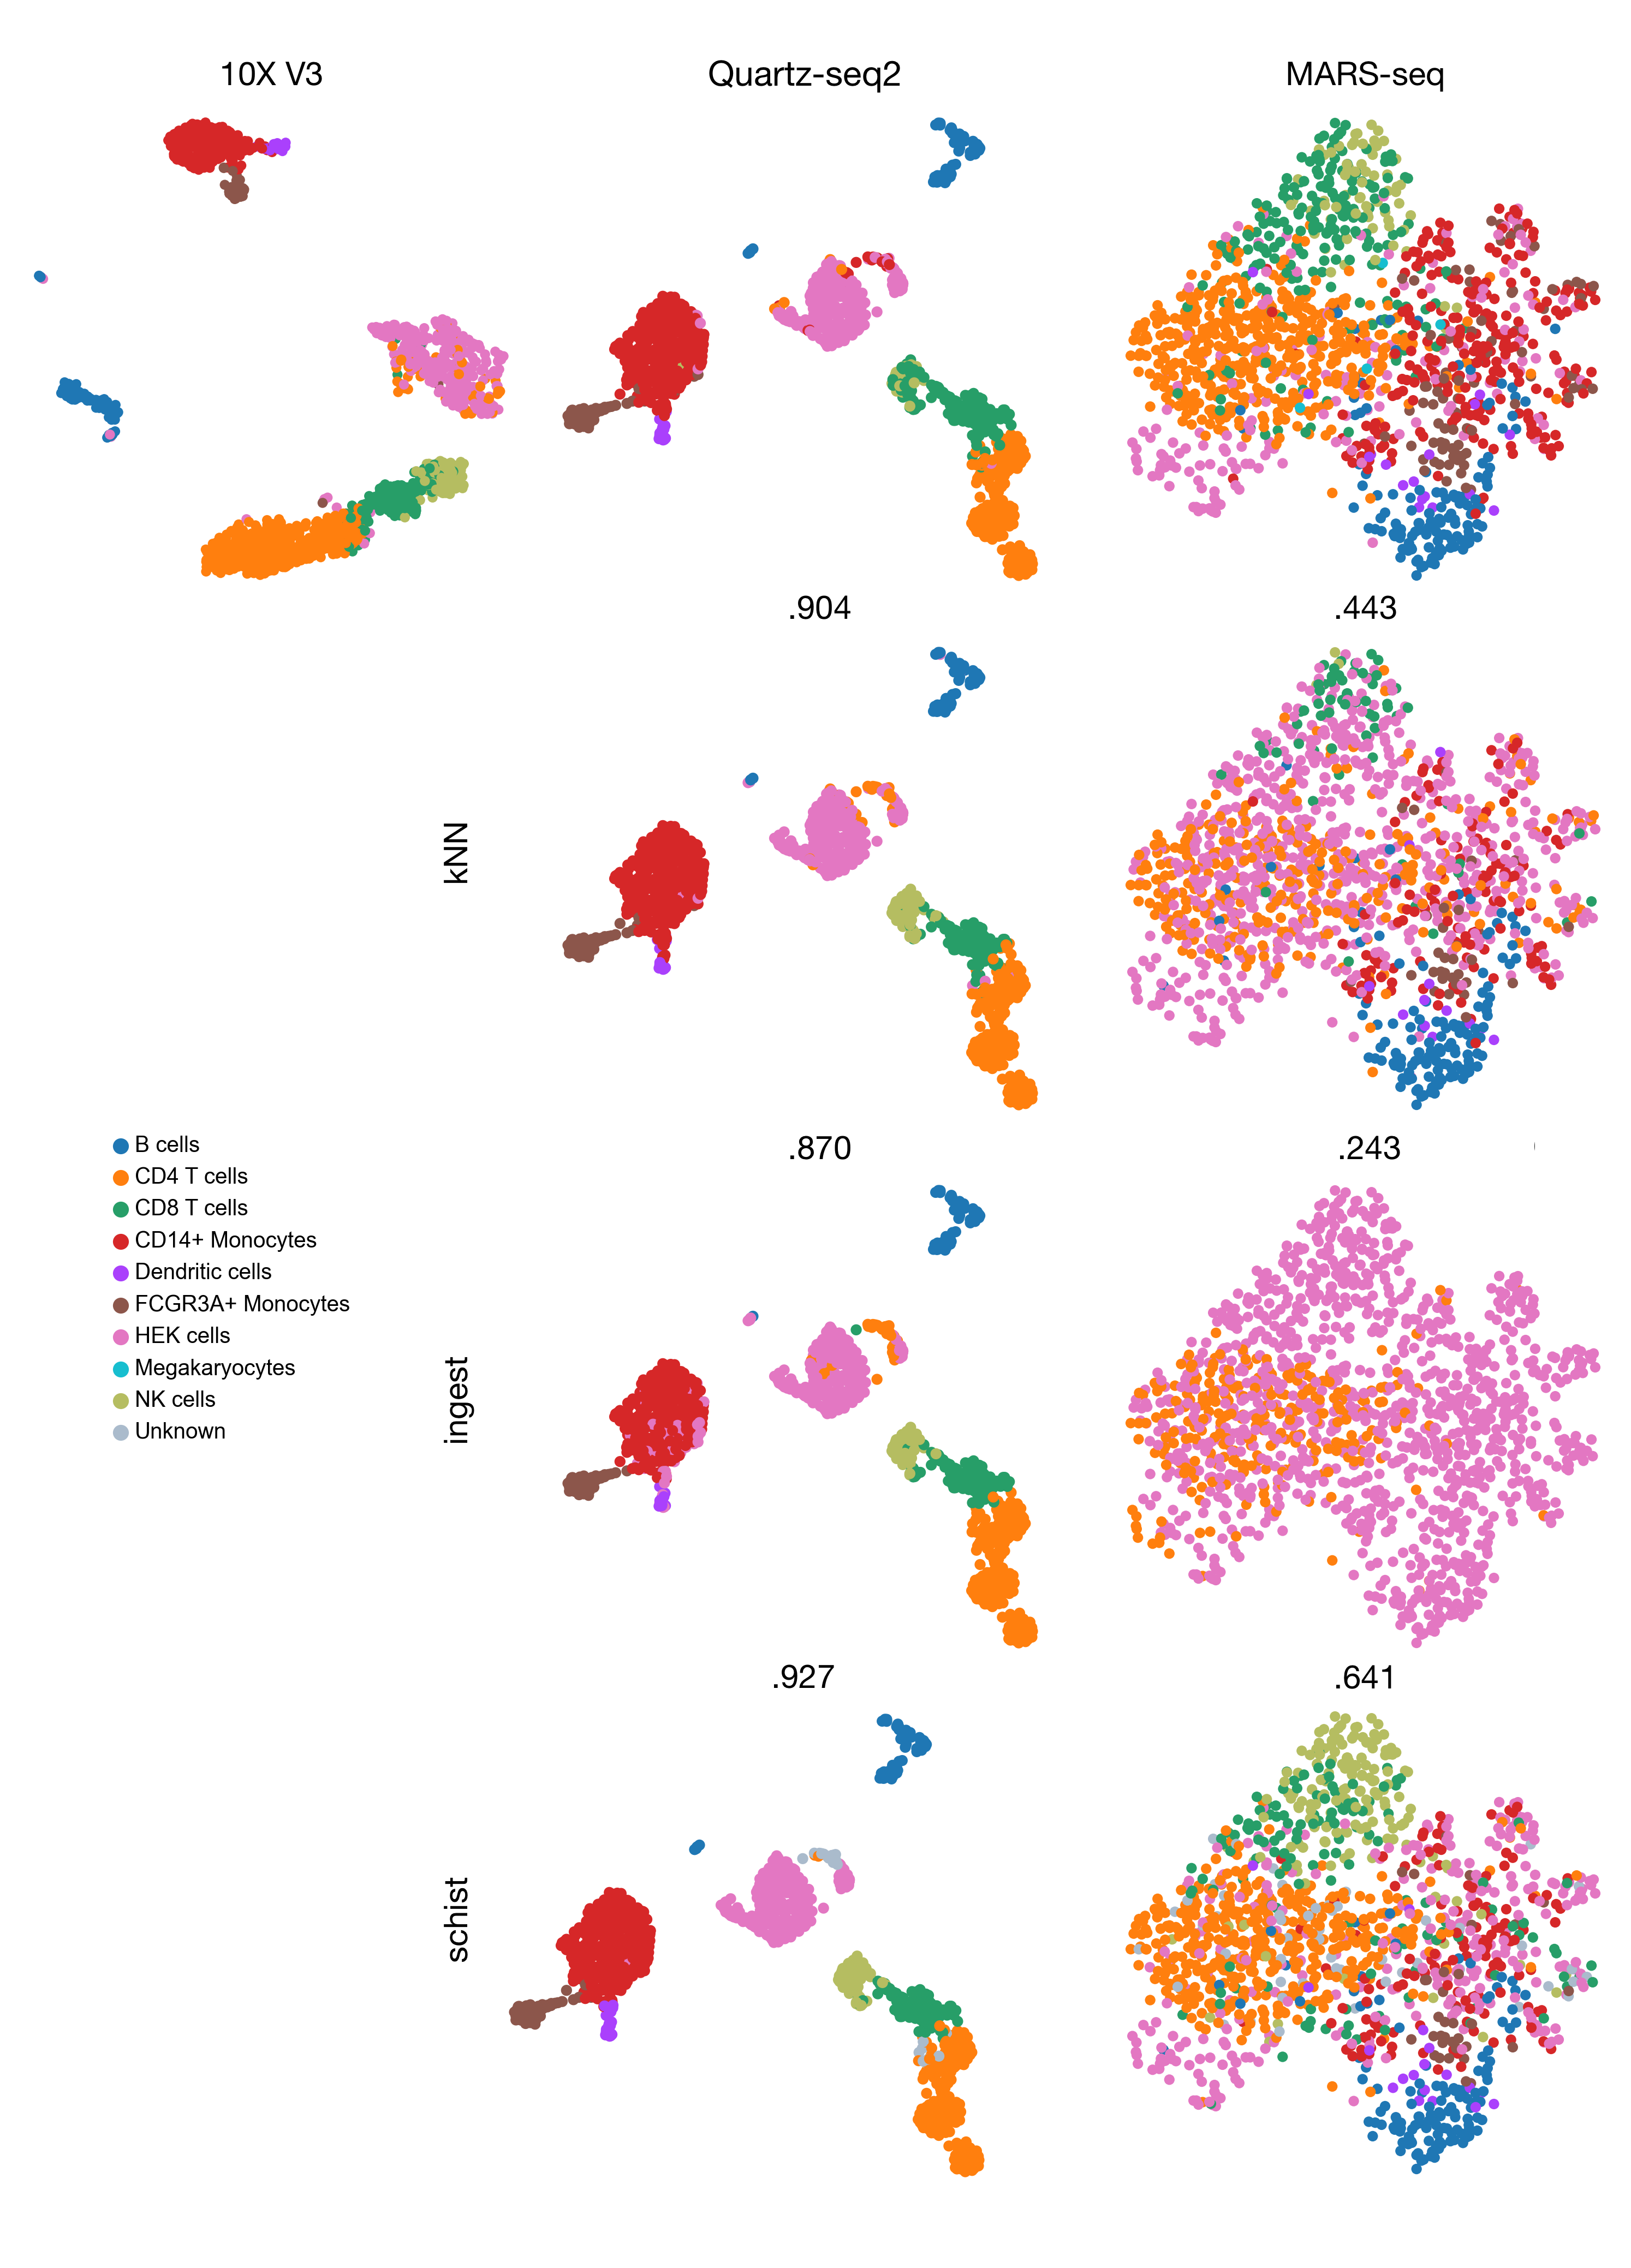
\includegraphics[keepaspectratio,width=\textwidth,height=0.55\textheight]{Figure_Label_Transfer.png}
\caption[]{Label transfer using SBM. Annotated data from Chromium 10X (A) and  MARS-seq (B) were merged using Harmony. MARS-seq cells were relabeled according to the \emph{k}NN graph (C) or by exploiting the Stochastic Block Model (D). }\label{Figure_Label_Transfer}
\end{figure}


\subsection*{Choice of the optimal level}

\textcolor{red}{TO BE DONE. Discuss modularity, but also eigenanalysis of random matrix}.

\subsection*{PPBM?}

\textcolor{red}{TO BE DONE. Maybe this is the right place to introduce the choice of the appropriate hierarchy level}


\subsection*{Analysis of runtimes}

\textcolor{red}{TO BE UPDATED WITH NEW DATA}

Minimisation of the nSBM is a process that may require a large amount of computational resources. The analysis of a relatively small scRNA-seq dataset, such as the ones in \cite{mereu_2020}, may require several minutes to be processed. This could be a serious limitation to the adoption of nSBM in the analysis of single cell data, especially because several parameters should be tested. To overcome this limitation, it was suggested to let a greedy merge-split MCMC algoritthm \cite{peixoto_2020} to explore the solutions and stop iterations when the difference in entropy is below a defined threshold. We tested this approach on a commodity hardware (MacBook Air, dual core 1.6 GHz i5 processor, 16 GB RAM) and compared to the default approach. Results are reported in Table \ref{Table1}. The merge-split algorithm greatly reduces the time needed to propose the final model. In addition, the partitions found are largely overlapping the ones found by the default approach. 

\begin{table}[h!]
\centering
 \begin{tabular}{|| l c c c c c ||}
%  \begin{tabular}{|| m{7em} | m{5em} | m{7em} | m{7em} | m{5em} ||}
 \hline
 \textbf{Dataset} & \textbf{Cells} & \textbf{Edges} & \textbf{Leiden} & \textbf{PPBM} & \textbf{NSBM} \\ [0.5ex] 
 \hline\hline
% sc-mixology \cite{tian_2019} & 860 & 01:11 & 00:03 & 0.884 \\ 
 %\hline
 Chromium 10x \cite{mereu_2020} & 1523 & 21447 & 00:24 & 01:34 & 03:29\\ 
 \hline
 Quartz-seq2 \cite{mereu_2020} & 1266 & 14603 & 00:16 & 00:30 & 02:10 \\
 \hline
 MARS-seq \cite{mereu_2020} & 1401 & 21756 & 00:24 & 01:10 & 06:11 \\
 \hline
 iCELL8 \cite{mereu_2020} & 1830 & 30636 & 00:34 & 01:31 & 09:06 \\
 \hline
 Paul15 \cite{paul_2015} & 2730 & 51475 & 01:21 & 03:35 & 12:17\\ 
 \hline
 Planaria \cite{plass_2018} & 21612 & 173667 & 06:32 & 34:12 & 3:17:08 \\
 \hline
% 4 & 545 & 18744 & 7560 \\
% \hline
% 5 & 88 & 788 & 6344 \\ [1ex] 
% \hline
\end{tabular}
\caption{Time required to minimise the nSBM using the default minimization method compared to the greedy merge-split MCMC. Times are expressed in mm:ss. Partition overlap measures concordance between the two models over the full hierarchy. Timing is the average after 3 initialisations.}
\label{Table1}
\end{table}

\section*{Conclusions}
\textcolor{red}{TO BE UPDATED}

Identification of cells sharing similar properties in single cell experiments is of paramount importance. A large number of approaches have been described, although the standardisation of analysis pipelines converged to methods that are based on modularity optimisation. We tackled the biological problem using a different approach, nSBM, which has several advantages over existing techniques. The most important advantage is the hierarchical definition of cell groups which eliminates the choice of an arbitrary threshold on clustering resolution. In addition, we showed that the hierarchy itself could have a biological interpretation, implying that the hierarchical model is a valid representation of the cell ensemble. Our approach introduces the evaluation of cluster consistency, which can be used to isolate cells with heterogeneous identity. Lastly, a statistical way to evaluate models is made available, allowing for reliable model selection. This last capability has the obvious advantage that the choice of parameters, hence the definition of cell clusters, could be conditioned to an evaluation metric which is robust and easy to understand (\emph{i.e.} the model entropy).

The major drawback of adopting this strategy is the substantial increase of runtimes. According to the developers of \emph{graph-tool}, runtimes are proportional to the number of edges in the neighbourhood graph and while it supports CPU-level parallelisation, a model minimisation is hundreds times slower than the extremely fast Leiden approach. Nevertheless, we show that a greedy merge-split MCMC algorithm can overcome this limitation, achieving performances that allow the usage of \emph{schist} on standard desktop hardware to analyse various single cell datasets.


\section*{Materials and Methods}

\subsection*{Analysis of Random data}
Data were retrieved in \emph{scanpy} environment using \emph{sc.datasets.pbmc3k\_processed()} function. The random \emph{k}NN graph was obtained shuffling the node labels of each edge. nSBM was performed with 3 initialisations using merge-split MCMC approach. UMAP embedding was recomputed after randomisation using the shuffled graph.


\subsection*{Analysis of cell mixtures}

Data and metadata for five cell mixture profiled by Chromium 10x were downloaded from the sc-mixology repository (\href{https://github.com/LuyiTian/sc_mixology}{https:/\slash github.com\slash LuyiTian\slash sc\_mixology}). Data were analysed using scanpy v1.4.6 \cite{wolf_2018}. Cells with less than 200 genes were excluded, as genes detected in less than 3 cells. Cells with less than 5\% of mitochondrial genes were retained for subsequent analysis. Data were normalised and log-transformed; number of genes and percentage of mitochondrial genes were regressed out. nSBM was initialised three times

\subsection*{Analysis of hematopoietic differentiation}

Data were retrieved using scanpy's built-in functions and were processed as in \cite{wolf_2019}, except for \emph{k}NN graph built using 30 principal components, 30 neighbours and diffmap as embedding. Gene signatures were calculated using the following gene lists
\begin{itemize}
\item Erythroids: Gata1, Klf1, Epor, Gypa, Hba-a2, Hba-a1, Spi1
\item Neutrophils, Elane, Cebpe, Ctsg, Mpo, Gfi1
\item Monocytes, Irf8, Csf1r, Ctsg, Mpo
\end{itemize}

nSBM was completed with 3 initialisations

\subsection*{Analysis of cluster consistency}

Count matrices were downloaded from GEO using the following accession numbers: GSE133535 (Chromium 10Xv3), GSE133543 (Quartz-seq2), GSE133542 (MARS-seq) and GSE133541 (iCELL8). Data were processed according to the methods in the original paper \cite{mereu_2020}. Briefly, cells with less than 10,000 total number of reads as well as the cells having less than 65\% of the reads mapped to their reference genome were discarded. Cells in the 95th percentile of the number of genes/cell and those having less than 25\% mitochondrial gene content were included in the downstream analyses. Genes that were expressed in less than five cells were removed. Data were normalized and log-transformed, highly variable genes were detected at minimal dispersion equal to 0.5. Neighbourhood graph was built using 30 principal components and 20 neighbours. nSBM was completed with 3 initialisations. 


\section*{Acknowledgements}

We would like to thank Tiago de Paula Peixoto (Central European University, ISI Foundation) and Giovanni Petri (ISI Foundation) for the discussions and the precious hints. We also would like to thank all people at COSR, in particular Giovanni Tonon and Paolo Provero.
This work has been supported by Accelerator Award: A26815 entitled:  "Single-cell cancer evolution in the clinic" funded through a partnership between Cancer Research UK and Fondazione AIRC




\bibliography{references}


\end{document}
